\documentclass[english,compress]{beamer} %,handout
\usepackage{amsmath}
\usepackage{graphicx}
\makeatletter

\usepackage{listings}
%\usetheme{Boadilla}
\usetheme{Warsaw}
\setbeamertemplate{footline}
{
  \leavevmode%
  \hbox{%
  \begin{beamercolorbox}[wd=.333333\paperwidth,ht=2.25ex,dp=1ex,center]{author in head/foot}%
\usebeamerfont{author in head/foot}\insertshortauthor~~(\insertshortinstitute)
  \end{beamercolorbox}%
  \begin{beamercolorbox}[wd=.333333\paperwidth,ht=2.25ex,dp=1ex,center]{title in head/foot}%
\usebeamerfont{title in head/foot}\insertshorttitle
  \end{beamercolorbox}%
  \begin{beamercolorbox}[wd=.333333\paperwidth,ht=2.25ex,dp=1ex,right]{date in head/foot}%
\usebeamerfont{date in head/foot}\insertshortdate{}\hspace*{2em}
\insertframenumber{} / \inserttotalframenumber\hspace*{2ex} 
  \end{beamercolorbox}}%
  \vskip0pt%
}
\setbeamercovered{transparent}
\defbeamertemplate{description item}{align left}{\insertdescriptionitem\hfill}
\usecolortheme[RGB={23,51,104}]{structure}

\usepackage{babel}

\begin{document}

\title[Master Thesis]{BlkKin: A Low-overhead tracing infrastructure \\
for software-defined storage systems}

\author{Marios-Evangelos Kogias}
\institute[CSLab NTUA]
{
  National Technical University of Athens \\
  School of Electrical and Computer Engineering
}

\chapter{Introduction}\label{ch:intro}

When back in April 1965 Gordon E. Moore stated the following 
\begin{quotation}
    ``The complexity for minimum component costs has increased at a rate of 
    roughly a factor of two per year. Certainly over the short term this rate 
    can be expected to continue, if not to increase. Over the longer term, the 
    rate of increase is a bit more uncertain, although there is no reason to 
    believe it will not remain nearly constant for at least 10 years. That 
    means by 1975, the number of components per integrated circuit for minimum 
    cost will be 65,000. I believe that such a large circuit can be built on a 
    single wafer.''\cite{Moore}
\end{quotation}

had no idea that he had actually started a race among the academia and the
industry to overcome or at least abide the this law.

At first, since the technology was premature, the evolution in VLSI technology
went hand in hand with the evolution in computer architecture. The more and
faster transistors resulted in achievements in instruction level parallelism
(ILP). From 1975 to 2005 the endeavour put in computer architecture resulted in 
technological advances varying from deeper pipelines and faster clock speeds to
superscalar architectures. But in around 2005 the ILP wall was hit. Transistors
could not be utilized to increase serial performance, logic became too complex
and performance attained was very low compared to power consumption. This lead
to the creation of multicore systems and entered the programmers to the jungle
of parallel software. So far the evolution was almost in accordance with the
famous law. However, in around 2009 to 2011, it was the power wall's time to be
hit. The famous power equation $P=cV^2f$ along with the CPU to memory gap
(eikona) led to the technological burst of distributed and cloud computing.

In 2009 Amazon.com introduced the Elastic Compute Cloud and since then the term
`cloud' is one of the hottest buzzwords not only among the industry and academia
but also among everyday people that take advantage of the `power of cloud'.
Although the term may be vague, the definition of cloud computing, according to
NIST (National Institute of Standards and Technology), is the following:

\begin{quotation}
    ``Cloud computing is a model for enabling ubiquitous, convenient, on-demand
    network access to a shared pool of configurable computing resources (e.g.,
    networks, servers, storage, applications, and services) that can be rapidly
    provisioned and released with minimal management effort or service provider
    interaction.  This cloud model is composed of five essential characteristics
    ,three service models, and four deployment models.''\cite{clouddef}
\end{quotation}

In the previous brief computer chronology, I kept describing bottlenecks and
walls to be overcome. However, it not clear how these bottlenecks become obvious
and how scientists can be sure that they have reached one's technology's limits
before moving on to the next one. The answer to the previous questions has
always been given through tracing. Tracing is a process recording information
about a program's execution, while it is being executed. These information may
be low level metrics like performance counters or time specific metrics in order
to evaluate system's latencies and throughput. Tracing data are mostly useful
for developers and can be used for debugging, performance tuning and performance
evaluation. From the single-cpu, integrated computer to the hundreds-node cloud
infrastructure, trace and performance engineers face challenging problems that
vary from platform to platform, but in any case play a vital role the system's
design and implementation.

Cloud and distributed computing provided trace engineers with more challenging
problems. The system scale is now much greater and program execution is far from
deterministic and can take place in any cluster node. So each program execution
is not bounded to a specific context. Other problems that needed solving
was data and time correlation between the different computing nodes. Also,
unlike single chip platforms that can be individually traced and evaluated,
cloud infrastructures need to be traced with full-load under production
conditions. This set more restrictions concerning the overhead that tracing adds
to the application. Finally, tracing is notorious about the amount of data that
produces. So distributed and cloud tracing demands the use of distributed data
storage systems and processing methods like distributed NOSQL databases and
Map-Reduce frameworks.

So to sum up, as described by any design model, the system verification consists
a major part of a system's implementation and working  process. Verification is
achieved through monitoring and tracing. Depending on the system's nature
tracing and monitoring process and the tools used may vary. Picking the right
tracing tools that will reveal the system's vulnerabilities and faults can be
very demanding and the performance engineer for bringing them to light,
respecting all the prerequisites set by the system.

\section{Thesis motivation}
The motivation behind this thesis emerged from concerns about the storage 
performance of the Synnefo \footnote{www.synnefo.org/} cloud software, which 
powers the \okeanos \footnote{https://okeanos.grnet.gr/} public cloud service 
\cite{okeanos}. I will briefly explain what \okeanos and Synnefo are in the 
following paragraphs.

\okeanos is an IaaS (Infrastructure as a Service) that provides Virtual 
Machines, Virtual Networks and Storage services to the Greek Academic and 
Research community. It is an open-source service that has been running in 
production servers since 2011 by GRNET S.A.
\footnote{Greek Research and Technology Network, https://www.grnet.gr/}

Synnefo \cite{synnefo} is a cloud software stack, also created by GRNET S.A., 
that implements the following services which are used by \okeanos:

\begin{itemize}
    \item \textit{Compute Service}, which is the service that enables the 
        creation and management of Virtual Machines.
    \item \textit{Network Service}, which is the service that provides network 
        management, creation and transparent support of various network 
        configurations.
    \item \textit{Storage Service}, which is the service responsible for 
        provisioning the VM volumes and storing user data.
    \item \textit{Image Service}, which is the service that handles the 
        customization and the deployment of OS images.
    \item \textit{Identity Service}, which is the service that is responsible 
        for user authentication and management, as well as for managing the 
        various quota and projects of the users.
\end{itemize}

Synnefo provides each virtual machine with at least one virtual volume
provisioned by the Volume Service called Archipelago\cite{archip-paper} and will
be furthered detailed in Chapter \label{}. This thesis' purpose is to provide
the developer or the system administrations with a cross-layer representation
accompanied with the equivalent metrics and time information of an I/O request's
route within the infrastructure from the time it is created inside the virtual
machine till it is finally served by the storage backend. The design and
implementation has to be done respecting the following two prerequisites:

\begin{itemize}
    \item The tracing information should be gathered and processed in real-time
        from every node participating in the request serving.
    \item The tracing infrastructure should add the least possible overhead to
        the instrumented system, which should continued working properly 
        production-wise
\end{itemize}

After the end of the tracing infrastructure implementation, the developer should
be able to identify the distinct phases and the duration of each that an IO
request passes through, measure communication latencies between the different
layers and collect all the necessary information (chosen by him) that would help
him understand the full context under which this specific request was served.
All these information can be used for software faults detection and performance
tuning as well as hardware malfunctions and faults like disk or network failures
that would be difficult to detect otherwise.

The novelty of this thesis consists in combining live cross-layer, multi-node
data aggregation, which is typical for monitoring but not for tracing, with the
precision and accuracy of tracing, respecting a hard prerequisite of low
overhead. Previous tracing infrastructures offered only partial solutions. Some
of them would separate the tracing from the working phase because of the great
added overhead, others provided no mechanism for data correlation, while the
traditional monitoring systems did not meet our low-level tracing needs.

The proposed system is called \textit BlkKin. It is designed respected the
aforementioned prerequisites and make use of the latest tracing semantics and
infrastructures employed by great tech companies like Google and Twitter.  

\section{Thesis structure} 
This thesis is structured as follows:

\section{Motivation}

\begin{frame}[t]{Outline}
\setcounter{tocdepth}{1}
\tableofcontents[currentsection]
\end{frame}

\subsection{Archipelago}
\begin{frame}{VM Volume storage}
\begin{center}
    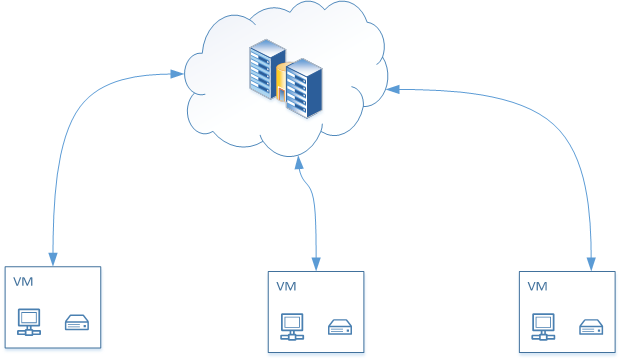
\includegraphics[scale=0.5]{images/cloud-storage.png} \\
\end{center}
\end{frame}

\begin{frame}{Archipelago I}
A thin distributed storage layer aiming to:
\hfill \\
\hfill \\
\hfill \\
\begin{itemize}
\item Decouple storage logic from the actual data store
\item Provide logic for thin cloning and snapshotting
\item Provide logic for deduplication
\item Provide different endpoint drivers to access Volumes and Files
\item Provide backend drivers for different storage technologies
\end{itemize}
\end{frame}

\begin{frame}{Archipelago II}
\begin{center}
    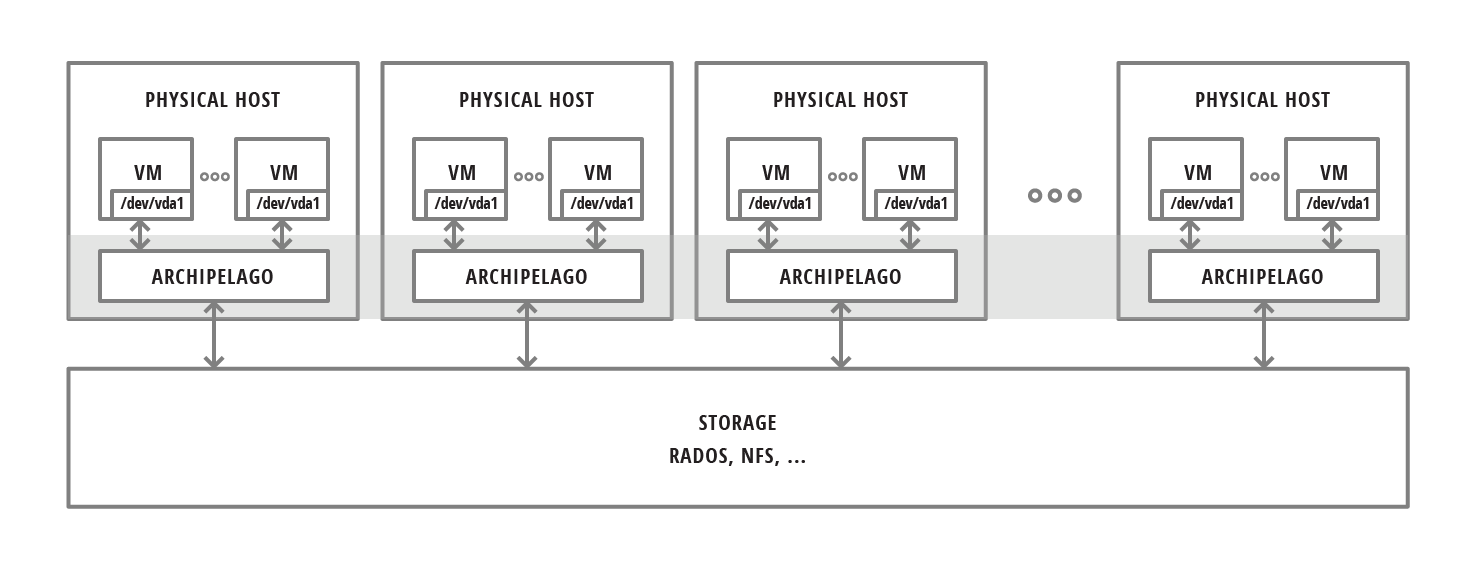
\includegraphics[scale=0.4]{images/archipelago-overview.png} \\
\end{center}
\end{frame}


\begin{frame}{Archipelago III}
\begin{center}
    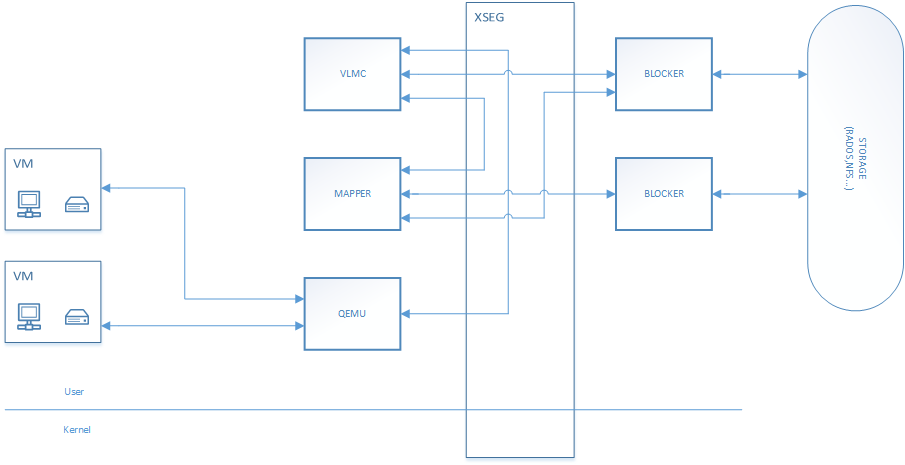
\includegraphics[scale=0.4]{images/archip-comm.png} \\
\end{center}
\end{frame}

\subsection{Distributed storage}

\begin{frame}{RADOS}
is the storage component of Ceph 
\hfill \\
\hfill \\
Ceph is a distributed object store and filesystem. 
\hfill \\
\hfill \\

RADOS basic characteristics are:
\begin{itemize}
\item Replication
\item Fault tolerance
\item Self-management
\item Scalability
\end{itemize}
\end{frame}


\begin{frame}{Storage Abstraction}
\begin{center}
    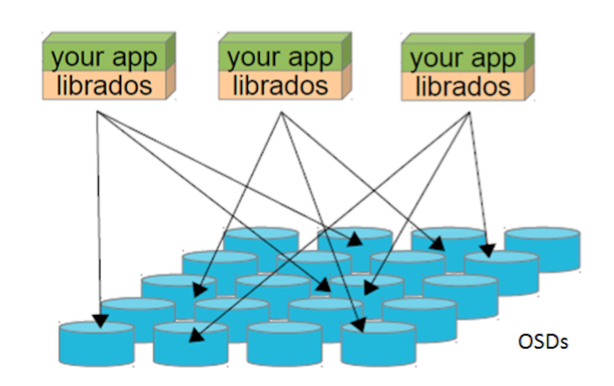
\includegraphics[scale=0.3]{images/rados_abstraction.png} \\
\end{center}
\end{frame}

\subsection{BlkKin}
\begin{frame}{The Problem}
\begin{itemize}
\item Complex service-oriented architectures
\item Difficult to debug
\item Difficult to monitor
\item Non-deterministic execution
\item Context-dependent faults
\end{itemize}
\end{frame}

\begin{frame}{Solution}
\begin{center}
Distributed end-to-end tracing 
\hfill \\
\hfill \\
 \& 
\hfill \\
\hfill \\
Central data collection
\end{center}
\end{frame}

\begin{frame}{BlkKin}

A distributed tracing infrastructure to track the I/O request from QEMU until
RADOS
\hfill \\
\hfill \\
\hfill \\

BlkKin's main characteristics:
\begin{itemize}
\item low-overhead tracing 
\item live-tracing
\item End-to-end tracing of causal relationships
\item User interface
\end{itemize}
\end{frame}

\chapter{Theoretical Background}\label{ch:bkg}

In this chapter we provide the necessary background to familiarize the reader
with the main concepts and mechanism used later in the document. For every
subsystem employed in BlkKin we briefly describe some counterparts justifying
our choice. The approach made is rudimentary, intended to introduce a reader
with elementary knowledge on distributed systems.

Specifically, Section \ref{sec:storage} covers the concepts around distributed
storage systems and the difficulties concerning their monitoring.  In Section
\ref{sec:archip-bkg} we describe Archipelago, Synnefo's Volume Service, and how
IO requests initiated within the virtual machine end up being served by a
distributed storage system. In Section \ref{sec:tracing-bkg} we explain the need
for tracing and cite various open-source tracing systems  with their advantages
and disadvantages. Finally, in Section \ref{sec:logging-bkg} we describe the
different needs covered by logging and cite some popular logging systems.


\section{Distributed storage systems}\label{sec:storage}

Providing reliable, high-performance storage that scales has been an ongoing
challenge for system designers. High-throughput and low-latency storage for file
systems, databases, and related abstractions are critical to the performance of
a broad range of applications. Historically, data centers first created
`islands' of SCSI disk arrays as direct-attached storage (DAS), each dedicated
to an application, and visible as a number of `virtual hard drives' (i.e.
LUNs). Initally, a SAN (Storage-Area-Network) consolidates such storage islands
together using a high-speed network. However, a SAN does not provide file
abstraction, only block-level operations. Also, the cost of scaling a SAN
infrastructure scales exponentially. These boosted the development of more
\emph{service-oriented-architectures}. Emerging clustered storage architectures
constructed from storage bricks or object storage devices (OSDs) seek to
distribute low-level block allocation decisions and security enforcement to
intelligent storage devices, simplifying data layout and eliminating I/O
bottlenecks by facilitating direct client access to data. OSDs constructed from
commodity components combine a CPU, network interface, and local cache with an
underlying disk or RAID, and replace the convention block-based storage
interface with one based on named, variable-length objects. As storage clusters
grow to thousands of devices or more, consistent management of data placement,
failure detection, and failure recovery places an increasingly large burden on
client, controller, or metadata directory nodes, limiting scalability.

One of the design principles of object storage is to abstract some of the lower
layers of storage away from the administrators and applications. Thus, data is
exposed and managed as objects instead of files or blocks. Objects contain
additional descriptive properties which can be used for better indexing or
management. Administrators do not have to perform lower level storage functions
like constructing and managing logical volumes to utilize disk capacity or
setting RAID levels to deal with disk failure. File metadata are explicitly
separate from data and data manipulation is allowed through programmatic
interfaces. These interfaces include CRUD functions for basic read, write and
delete operations, while some object storage implementations go further,
supporting additional functionality like object versioning, object replication,
and movement of objects between different tiers and types of storage. Most API
implementations are ReST-based, allowing the use of many standard HTTP calls.
This results in the abstraction shown in Figure
\ref{fig:object_storage_arch.png}.
 
\diagram{Storage Abstraction}{object_storage_arch.png}

Alhtough they differ substantially concerning their implementation, some of the
most popular examples of such systems are: Amazon S3, OpenStack Swift and RADOS.

However, one common characteristic of all these systems, that led to the
development of this thesis, is that they provide an architecture that easily
scales out, based on APIs, but which is difficult to monitor and find out what
really went wrong in case of a problem. This leads to a di-centralized data
collection and a centralized data processing architecture for tracing
information which is further explained in Chapter \ref{}.

\subsection{RADOS}\label{sec:rados}
RADOS stands for  Reliable, Autonomic Distributed Object Store. It is the object
store component of Ceph\footnote{http://ceph.com/}.Ceph is a free distributed
object store and file system that has been created by Sage Weil for his doctoral
dissertationi\cite{weil-thesis} and has been supported by his company, Inktank,
ever since.  RADOS seeks to leverage device intelligence to distribute the
complexity surrounding consistent data access, redundant storage, failure
detection, and failure recovery in clusters consisting of many thousands of
storage devices.

RADOS basic characteristics are:
\begin{itemize}
\item \textit{Replication}, which means that there can be many copies
of the same object so that the object is always accessible,
even when a node experiences a failure.
\item \textit{Fault tolerance}, which is achieved by not having a
single point of failure. Instead, RADOS uses elected servers
called \textbf{monitors}, each of which have mappings of the
storage nodes where the objects and their replicas are stored.
\item \textit{Self-management}, which is possible since monitors know
at any time the status of the storage nodes and, for example,
can command to create new object replicas if a node experiences
a failure.
\item \textit{Scalability}, which is aided by the fact that there is no
point of failure, which means that adding new nodes
theoretically does not add any communication overhead.
\end{itemize}

Ceph's building blocks can be seen in Figure \ref{fig:ceph.png}

\diagram{Ceph abstraction}{ceph.png}

RADOS operations are based on the following components:
\begin{itemize}
    \item \textit{object store daemons}, which are userspace processes that run 
        in the storage backend and are responsible for storing the data.
    \item \textit{monitor daemons}, which are monitoring userspace processes 
        that run in an odd number of servers that form a Paxos part-time 
        parliament\cite{Paxos}. Their main responsibility is holding and 
        reliably updating the mapping of objects to object store daemons, as 
        well as self-healing when an object store daemon or monitor daemon has 
        crashed.
\end{itemize}

Ceph's logic is based on \textit CRUSH algorithm. According to this algorithm a
map is created, called CRUSH map, which maps objects to store daemons. A
fundamental idea in RADOS is the \textit{placement group} (pg). Placement groups
are used for load balancing. The number of placement groups is predefined. Then,
when we want to create a new object, its name is hashed and assigned to a
specific group. Each placement group makes IO requests to the same OSDs. So,
objects belonging to the same pg, will be replicated across the same OSDs. The
relationship between placement groups and object store daemons is stored in
CRUSH maps that each monitor daemon holds.   
  
Since we would like to instrument RADOS code and measure its performance, apart
from the theoretical background, we should also explain some of its operating
internals, so that further analysis is consolidated. So, in brief, we will try
to explain an IO request's route within a RADOS infrastructure.

Although, as seen in Figure \ref{fig:ceph.png}, RADOS has multiple entry points
(RBD, CephFS, RADOSGW), we are interested in the interaction with librados.
Librados provides a well defined API for data manipulation and control, namely
an API that enables to modify (CRUD) objects and interact with the Ceph
monitors. There are binding for various languages like C, Python and Java. 

Hypothetically, we have an application using librados, which can also run
remotely from the RADOS cluster. The application want to write an objects. So, a
nIO request is initiated from librados. RADOS employs an asynchronous, ordered
point to point message passing library for communication. So, this request is
serialized and a TCP message is created and sent to the RADOS cluster. After
receive, this packet is handled by the equivalent RADOS Messenger classes,
decoded and based on its kind, is placed in a \textit{dispatch queue} to be
served. This specific object belongs to a specific placement group. So, when the
request reaches the top of the queue, based on this pg, the equivalent OSD
undertakes its serving. Based on the replication factor, the equivalent number
of replication requests is sent to other OSDs responsible for the same pg.
During request handling per OSD, based on the request type, there are phases
like \textit{Journal Access} and finally the \textit{Filestore Access}.

From the above analysis, we understood that request processing in RADOS is a
perplexed procedure including multiple remote nodes collaborating. The only way
to understand the internals and debug possible latencies and bottlenecks is
through tracing and this is what we are going to examine further in this thesis.

\section{Archipelago}\label{sec:archip-bkg}

\section{Tracing Systems}\label{sec:tracing-bkg}
Understanding where time has been spent in performing a computation or servicing
a request is at the forefront of the performance analyst’s mind. Measurements
are available from every layer of a computing system, from the lowest level of
the hardware up to the top of the distributed application stack. In recent years
we have seen the emergence of tools which can be used to directly trace events
relevant to performance. This is augmenting the traditional event count and
system state instrumentation, and together they can provide a very detailed view
of activity in the complex computing systems prevalent today.

Event tracing has the advantage of keeping the performance data tied to the
individual requests, allowing deep inspection of a request which is useful when
performance problems arise. The technique is also exceptionally well suited to
exposing transient latency problems. The downsides are increased overheads
(sometimes significantly) in terms of instrumentation costs as well as volumes
of information produced. To address this, every effort is taken to reduce the
cost of tracing - it is common for tracing to be enabled only conditionally, or
even dynamically inserted into the instrumented software and removed when no
longer being used.

In early 1994, a technique called dynamic instrumentation or Dyninst API
\cite{dynist} was
proposed to provide efficient, scalable and detailed data collection for
large-scale parallel applications (Hollingsworth et al., 1994). Being one of the
first tracing systems, the infrastructure built for data extraction was limited.
The operating systems at hand were not able to provide efficient services for
data extraction. They had to build a data transport component to read the
tracing data, using the ptrace function, that was based on a time slice to read
data. A time slice handler was called at the end of each time slice, i.e when
the program was scheduled out, and the data would be read by the data transport
program built on top.

This framework made possible new tools like DynaProf \cite{dynaprof} and
graphical user interface for data analysis. DynaProf is a dynamic profiling tool
that provides a command line interface, similar to gdb, used to interact with
the DPCL API and to basically control tracing all over your system.

Kernel tracing brought a new dimension to infrastructure design, having the
problem of extracting data out of the kernel memory space to make it available
in user-space for analysis. The K42 project \cite{k42}  used shared
buffers between kernel and user space memory, which had obvious security issues.
A provided daemon waked up periodically and emptied out the buffers where all
client trace control had to go through. This project was a research prototype
aimed at improving tracing performance. Usability and security was simply
sacrificed for the proof of concept. For example, a traced application could
write to these shared buffers and read or corrupt the tracing data for another
application, belonging to another user.

In the next sections, recent tracers and how they built their tracing
infrastructure will be examined.

\subsection{Magpie}

One of the earliest and most comprehensive event tracing frameworks is Magpie
\cite{magpie}.  This project builds on the Event Tracing for Windows
infrastructure which underlies all event tracing on the Microsoft Windows
platform. Magpie is aimed primarily at workload modelling and focuses on
tracking the paths taken by application level requests right through a system.
This is implemented through an instrumentation framework with accurate and
coordinated timestamp generation between user and kernel space, and with the
ability to associate resource utilisation information with individual events.

The Magpie literature demonstrates not only the ability to construct high-level
models of a distributed system resource utilisation driven via Magpie event
tracking, but also provides case studies of low-level performance analysis,
such as diagnosing anomalies in individual device driver performance. Magpie
utilises a novel concept in behavioural clustering, where requests with similar
behaviour (in terms of temporal alignment and resource consumption) are
grouped. This clustering underlies the workload modelling capability, with each
cluster containing a group of requests, a measure of “cluster diameter”, and
one selected “representative request” or “centroid”. The calculation of cluster
diameter indicates deep event knowledge and inspection capabilities, and
although not expanded on it implies detailed knowledge of individual types of
events and their parameters. This indicates a need for significant user
intervention to extend the system beyond standard operating system level
events.

As an aside, it is worth noting here that, for the first time, we see in Magpie
the use of a binary tree graph to represent the flow of control between events
and sub-events across distinct client/server processes and/or hosts.

\subsection{DTrace}
Then, Sun Microsystemsa released, in 2005, DTrace \cite{dtrace} which offers the
ability to dynamically instrument both user-level and kernel-level software. As
part of a mass effort by Sun, a lot of tracepoints were added to the Solaris 10
kernel and user space applications. Projects like FreeBSD and NetBSD also ported
dtrace to their platform, as later did Mac OS X. The goal was to help developers
find serious performance problems. The intent was to deploy it across all
Solaris servers and to use it in production.  If we look at the DTrace
architecture, it uses multiple data providers, which are basically probes used
to gather tracing data and write it to memory buffers.  The framework provides a
user space library (libdtrace) which interacts with the tracer through ioctl
system calls. Through those calls, the DTrace kernel framework returns specific
crafted data for immediate analysis by the dtrace command line tool. Thus, every
interaction with the DTrace tracer is made through the kernel, even user space
tracing.  On a security aspect, groups were made available for different level
of user privileges. You have to be in the dtrace proc group to trace your own
applications and in the dtrace kernel group to trace the kernel.  A third group,
dtrace user, permits only system call tracing and profiling of the user own
processes.  This work was an important step forward in managing tracing in
current operating systems in production environment. The choice of going through
the kernel, even for user space tracing, is a performance trade-off between
security and usability.

\subsection{SystemTap}
In early 2005, Red Hat released SystemTap \cite{systemtap} which also
offers dynamic instrumentation of the Linux kernel and user applications. In
order to trace, the user needs to write scripts which are loaded in a tapset
library. SystemTap then translates these in C code to create a kernel module.
Once loaded, the module provides tracing data to user space for analysis.
Two system groups namely stapdev and stapusr are available to separate possible
trac- ing actions. The stapdev group can do any action over Systemtap
facilities, which makes it the administrative group for all tracing control (Don
Domingo, 2010) and module creation.
The second group, stapusr, can only load already compiled modules located in
specific protected directories which only contain certified modules.
The project also provides a compile-server which listens for secure TCP/IP
connections using SSL and handles module compilation requests from any certified
client. This acts as a SystemTap central module registry to authenticate and
validate kernel modules before loading them.
This has a very limited security scheme for two reasons. First, privileged
rights are still needed for specific task like running the compilation server
and loading the modules, since the tool provided by Systemtap is set with the
setuid bit. Secondly, for user space tracing, only users in SystemTap’s group
are able to trace their own application, which implies that a privileged user
has to add individual users to at least the stapusr group at some point in time,
creating important user management overhead.
It is worth noting that the compilation server acts mostly as a security barrier
for kernel module control. However, like DTrace, the problem remains that it
still relies on the kernel for all tracing actions. Therefore, there is still a
bottleneck on performance if we consider that a production system could have
hundreds of instrumented applications tracing simultaneously. This back and
forth in the kernel, for tracing control and data retrieval, cannot possibly
scale well.

\section{Logging Systems}\label{sec:logging-bkg}

Logs are a critical part of any system, they give you insight into what a system
is doing as well what happened. Unlike tracing, log data are not low-level and
do not refer to the system's performance and there is no special care about the
overhead that logging add to the system. Virtually every process running on a
system generates logs in some form or another. Usually, these logs are written
to files on local disks. When your system grows to multiple hosts, managing the
logs and accessing them can get complicated. Searching for a particular error
across hundreds of log files on hundreds of servers is difficult without good
tools. A common approach to this problem is to setup a centralized logging
solution so that multiple logs can be aggregated in a central location.

There are various options for log data aggregation as well as for visualizing
the aggregated data. Some of them are cited here:

\subsection{Syslog}

Syslog is a standard for computer message logging. It permits separation of the
software that generates messages from the system that stores them and the
software that reports and analyzes them.

Syslog can be used for computer system management and security auditing as well
as generalized informational, analysis, and debugging messages. It is supported
by a wide variety of devices (like printers and routers) and receivers across
multiple platforms. Because of this, syslog can be used to integrate log data
from many different types of systems into a central repository.

Messages are labeled with a facility code (one of: auth, authpriv, daemon, cron,
ftp, lpr, kern, mail, news, syslog, user, uucp, local0 ... local7) indicating
the type of software that generated the messages, and are assigned a severity
(one of: Emergency, Alert, Critical, Error, Warning, Notice, Info, Debug).

Implementations are available for many operating systems. Specific configuration
may permit directing messages to various devices (console), files (/var/log/) or
remote syslog servers. Most implementations also provide a command line utility,
often called logger, that can send messages to the syslog. Some implementations
permit the filtering and display of syslog messages.

Syslog is standardized by the IETF in RFC 5424. This standardization specifies a
very important characteristic of Syslog that we would like to have available in
our tracing infrastructure and this is severity levels. Every event to be traced
is associated with a severity level varying from Emergency when the system is
unusable to informational or debug level messages. From the syslog side the
administrator can define which events he is interested about. So, for testing
environments more events should be traced, while for production environments the
events to be traced should be restricted to the absolutely needed. 

\subsection{Scribe}
A new class of solutions that have come about have been designed for high-volume
and high-throughput log and event collection. Most of these solutions are more
general purpose event streaming and processing systems and logging is just one
use case that can be solved using them. They generally consist of logging
clients and/or agents on each specific host. The agents forward logs to a
cluster of collectors which in turn forward the messages to a scalable storage
tier. The idea is that the collection tier is horizontally scalable to grow with
the increase number of logging hosts and messages. Similarly, the storage tier
is also intended to scale horizontally to grow with increased volume. This is
gross simplification of all of these tools but they are a step beyond
traditional syslog options.

One popular solution is
Scribe\footnote{https://github.com/facebookarchive/scribe}. Scribe is a server
for aggregating log data that's streamed in real time from clients. It is
designed to be scalable and reliable.  It was used and released by Facebook as
open source. Scribe is written in C++ and it worths mentioning its transport
layer and how Scribe logging data are processed and finally stored.

Concerning its \textbf{transport} layer, Scribe uses
Thrift\footnote{https://thrift.apache.org/}. The Apache Thrift software
framework, for scalable cross-language services development, combines a software
stack with a code generation engine to build services that work efficiently and
seamlessly between different programming languages. After describing the service
in a specific file (thrift file), the framework is  responsible for generating
the code to be used to easily build RPC clients and servers that communicate
seamlessly across programming languages. For Scribe especially the thrift file
is the following:  

\ccode{Scribe thrift definition file}{scribe.thrift}

In the above file a \texttt Log method is defined, which takes a list of
\texttt LogEntry items as parameter. Every \texttt LogEntry consists of two
strings, a category and a message. This specific Log method can return two
different results codes, either `OK' or `TRY\_LATER'. Based on this file, using
Thrift we can create Scribe clients for every programming language.

Concerning \textbf{data manipulation} Scribe provides the following options.
Based on the message's category, it can store the log entries in different
files, one per category. Also Scribe has Hadoop support and can store the
tracing information to an HDFS so that they can be processed later using
Map-Reduce jobs.

Scribe servers are arranged in a directed graph, with each server
knowing only about the next server in the graph. This network topology allows
for adding extra layers of fan-in, as a system grows and batching messages
before sending them between datacenters as well as providing reliability in case
of intermittent connectivity or node failure. So a Scribe server can operate
either as a terminal server where data are finally stored, or as an intermediate
server that forwards data to the next Scribe server. In case of congestion or of
network problems, data are stored locally and forwarded when the problem is
restored.

\subsection{Graphite} 
Graphite is an enterprise-scale monitoring tool that runs well on cheap
hardware. It is released under the open source Apache 2.0 license and it is
used by many big companies like Google and Canonical. Although Graphite is not
responsible for collecting data, it can store efficiently numeric time-series
data and render graphs of this data on demand. Graphite can cooperate with other
tools like collectd\footnote{https://collectd.org/} for data aggregation.

From an architectural aspect, Graphite consists of 3 software components:

\begin{description}
\item[carbon] - a Twisted daemon that listens for time-series data
\item[whisper] - a simple database library for storing time-series data (similar
in design to RRD)
\item[graphite webapp] - A Django webapp that renders graphs on-demand using
Cairo\footnote{http://www.cairographics.org/}
\end{description}

\subsection{Ganglia}
Ganglia\cite{ganglia} is a scalable distributed monitoring system for high performance
computing systems such as clusters and Grids and grew out of the University of
California, Berkeley. It is based on a hierarchical design targeted at
federations of clusters. It relies on a multicast-based listen/announce protocol
to monitor state within clusters and uses a tree of point-to-point connections
amongst representative cluster nodes to federate clusters and aggregate their
state. It leverages widely used technologies such as XMLfor data representation,
XDR for compact, portable data transport, and RRDtool for data storage and
visualization. It uses carefully engineered data structures and algorithms to
achieve very low per-node overheads and high concurrency. The implementation is
robust, has been ported to an extensive set of operating systems and processor
architectures, and is currently in use on over 500 clusters around the world. 

\diagram{Ganglia architecture}{ganglia-architecture.png}

Ganglia architecture is made up of the following components.

\begin{description}

\item[gmond] The Ganglia MONitor Daemon is a data-collecting agent that you must
install on every node in a cluster. Gmond gathers metrics about the local node
and sends information to other nodes via XML to a browser window. Gmond is
portable and collects system metrics, such as CPU, memory, disk, network and
process data. The Gmond configuration file /etc/gmond.conf controls the Gmond
daemon and resides on each node where Gmond is installed.
    
\item[gmetad] The Ganglia METAdata Daemon is a data-consolidating agent that
provides a query mechanism for collecting historical information about groups of
machines. Gmetad is typically installed on a single, task-oriented server (the
monitoring node), though very large clusters could require more than one Gmetad
daemon. Gmetad collects data from other Gmetad and Gmond sources and stores
their state in indexed RRDtool (round-robin) databases, where a Web interface
reads and returns information about the cluster. The Gmetad configuration file
/etc/gmetad.conf controls the Gmetad daemon and resides on the monitoring node.
    
\item[RRDtool] RRDTool is an open-source data logging and graphing system that
Ganglia uses to store the collected data and to render the graphs for Web-based
reports. Cron jobs that run in the background to collect information from the HP
Vertica monitoring system tables are stored in the RRD database.
    
\item[PHP-based Web interface] — The PHP-based Web interface contains a
collection of scripts that both the Ganglia Web reporting front end and the HP
Vertica extensions use. The Web server starts these scripts, which then collect
HP Vertica‑specific metrics from the RRD database and generate the XML graphs.
These scripts provide access to HP Vertica health across the cluster, as well as
on each host.

\item[Web server] The Web server uses lighttpd, a lightweight http server that
can be any Web server that supports PHP, SSL, and XML. The Ganglia web front end
displays the data stored by Gmetad in a graphical web interface using PHP.
\item[Advanced tools] Gmetric, an executable, is added during Ganglia
installation. Gmetric provides additional statistics and is used to store
user-defined metrics, such as numbers or strings with units.

\end{description}

\section{Conclusion}
To sum up, it is obvious from the previous analysis that the tracing systems
mentioned do not fit in our demands concerning the added overhead to the
instrumented application since their solutions pass through the kernel space.
This extra overhead makes them unsuitable for live tracing. The solution for
for the BlkKin tracing backend was given from the Linux Trace Toolkit - next
generation (LTTng) because it provides separate mechanisms for kernel and user
space tracing. LTTng is furthered examined in Chapter \ref{}.

Concerning the logging systems, we need to imitate their architecture for
BlkKin's architecture, since we need a central trace aggragation point and a UI
that visualizes the information. We can conclude that we need:
\begin{itemize}
\item[tracing daemon] that runs on every cluster node and collects data  with a low-overhead
\item[central data collector] where all tracing information are stored
\item[Web UI] where tracing information are rendered in a way that extracts the necessary
information revealing problems and performance issues in the first place.
For more elaborate information extraction, trace information can be furthered
processed apart from the UI.  
\end{itemize}
For data collection, we are going to use LTTng, while for the data aggregation and the visualization we
are going to use Zipkin, a distributed tracing system created by Twitter. Zipkin
as well as the reasons for our choice are furthered examined in Chapter \ref{}.

\end{document}
